\chapter{Runoff generation} \label{chap:runGen}
\renewcommand{\tabdir}{chapters/part_processes/runoffGeneration/tab}
\renewcommand{\figdir}{chapters/part_processes/runoffGeneration/fig}

\section{Introduction} \label{sec:runGen_intro}

To avoid confusion, it is important to distinguish between the terms \emph{runoff generation} and \emph{runoff concentration}. As \emph{runoff generation}, we understand the transformation of water input (rain, snow melt) into runoff \emph{at the local scale}, \ie{} at every single point of a catchment. In contrast to that, the term \emph{runoff concentration} describes the transport of the locally generated runoff to the catchment's outlet (or the nearest river).

In some cases, the strict separation of the two terms is really pragmatic. However, it provides a clear and quite useful concept for hydrological catchment modeling.

%%%%%%%%%%%%%%%%%%%%%%%%%%%%%%%%%%%%%%%%%%%%%%%%%%%%%%%%%%%%%%%%%%%%%%%%%%%%%%%%
%%%%%%%%%%%%%%%%%%%%%%%%%%%%%%%%%%%%%%%%%%%%%%%%%%%%%%%%%%%%%%%%%%%%%%%%%%%%%%%%
%%%%%%%%%%%%%%%%%%%%%%%%%%%%%%%%%%%%%%%%%%%%%%%%%%%%%%%%%%%%%%%%%%%%%%%%%%%%%%%%

\section{Simple four components model} \label{sec:runGen4comp}

%%%%%%%%%%%%%%%%%%%%%%%%%%%%%%%%%%%%%%%%%%%%%%%%%%%%%%%%%%%%%%%%%%%%%%%%%%%%%%%%

\subsection{Processes and equations} \label{sec:runGen4comp_processes}

The four components runoff generation model described here is based on the concepts used in the LARSIM\footnote{Model variant '4Q-KOMP mit A2'} model \citet{Ludwig2006}. Originally, most equations were first presented by \citet{Todini1996}.

The runoff generation model is built upon the water balance of a soil column (\figref{fig:runGen4comp_soilWater}) which can be expressed by \eqnref{eqn:runGen4comp_soilWaterBalance}

\begin{equation} \label{eqn:runGen4comp_soilWaterBalance}
  \frac{d\soilWaterContent}{dt} = \frac{\rateWaterSupply - \rateRunoffSurf - \rateRunoffPref - \rateRunoffInter - \rateRunoffBase - \rateEvapotransp}{\soilDepth}
\end{equation}

with

\begin{tabular}{llp{0.6\columnwidth}}
\soilWaterContent & (--) & Soil water content as \cbm/\cbm \\
\rateWaterSupply & (m/s) & Rate of water supply (see \eqnref{eqn:runGen4comp_waterSupply}) \\
\rateRunoffSurf & (m/s) & Rate of surface runoff \\
\rateRunoffPref & (m/s) & Rate of quick sub-surface runoff (preferential flow) \\
\rateRunoffInter & (m/s) & Rate of slow sub-surface runoff (interflow) \\
\rateRunoffBase & (m/s) & Rate of deep percolation (rate of ground water recharge) \\
\rateEvapotransp & (m/s) & Rate of evapo(transpi)ration \\
\soilDepth & (m) & Depth (thickness) of soil column. \\
\end{tabular}

\medskip
The relevant thickness of the soil column \soilDepth{} is equivalent to the rooted depth. Soil water at greater depths is assumed (1) to be unavailable for evapotranspiration and (2) not to contribute to lateral runoff processes.

\begin{figure}
  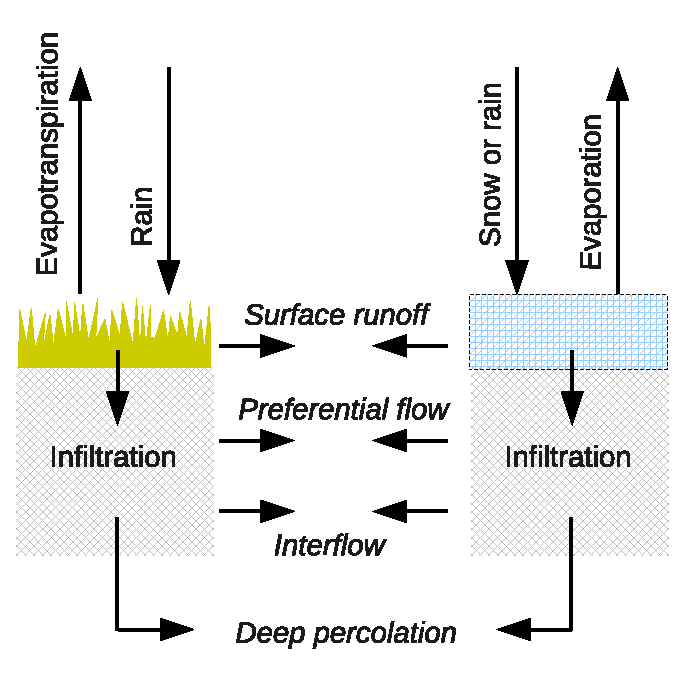
\includegraphics[width=0.9\columnwidth]{\figdir/soilWaterFluxes.eps}
  \caption{Water fluxes with respect to a soil column with (right) and without snow cover (left). \label{fig:runGen4comp_soilWater}}
\end{figure}

Snow coverage of the soil column is assumed to be either 0 or 100\%, \ie{} partial covering is \emph{not} simulated. As long as no snow is present, the rate of water supply to the soil column is the same as the intensity of precipitation, \precipIntensity{}. Once a snow cover exists, all precipitation is trapped in the snow and the rate of water supply is controlled by the melt rate, \rateSnowMelt{} (\eqnref{eqn:runGen4comp_waterSupply}). Both \precipIntensity{} and \rateSnowMelt{} are in units of m/s.

\begin{align} \label{eqn:runGen4comp_waterSupply}
  \rateWaterSupply =
  \begin{cases}
    \rateSnowMelt & \text{if snow cover is present} \\
    \precipIntensity & \text{else} \\
  \end{cases}
\end{align}

In the presented four components model, the generation of direct runoff\footnote{Runoff being quickly generated in response to water input.} is bound to the existence of (local) soil saturation. Thus, the model accounts for surface runoff due to infiltration excess but \emph{not} for Hortonian surface runoff.

Following to the Xinanjiang approach \citep{Zhao1980}, the fraction of saturated areas \satFrac{} in a catchment can be estimated from the area-integrated relative saturation of the soil \relSat{} which is the ratio of the current and maximum soil water content \soilWaterContent{} and \soilWaterContentMax{}, respectively (\eqnsref{eqn:runGen4comp_relativeSaturation} and \ref{eqn:runGen4comp_satFrac}). The rationale of the Xinanjiang model is a positive correlation between the catchment's average wetness, represented by the relative filling of the soil reservoir and the proportion of saturated areas. In other words, the occurrence of local saturation is assumed to increases as the catchment's average wetness becomes higher.

\begin{align}
  \relSat =& \frac{\soilWaterContent}{\soilWaterContentMax} \label{eqn:runGen4comp_relativeSaturation} \\
  \satFrac=& 1 - \left( 1 - \relSat \right) ^ \expSatFrac \label{eqn:runGen4comp_satFrac}
\end{align}

The shape of the relation between \relSat{} and \satFrac{} is controlled by a dimensionless empirical parameter \expSatFrac{}. The effect of different values of \expSatFrac{} is illustrated in \figref{fig:runGen4comp_expSatFrac}. A linear relation is assumed in the case $\expSatFrac{}=1$. Note that only values of $\expSatFrac{} \le 1$ are physically reasonable.
Max
\begin{figure}
  \includegraphics[width=0.9\columnwidth,angle=270]{\figdir/xinanjiang.eps}
  \caption[Influence of the empirical parameter \expSatFrac{}.]{Influence of the empirical parameter \expSatFrac{} on the relation between the catchment-integrated relative filling of the soil reservoir (x-axis) and the fraction of saturated areas \satFrac{} (y-axis). Only values of $\expSatFrac{} \le 1$ are physically reasonable. \label{fig:runGen4comp_expSatFrac}}
\end{figure}

The amount of direct runoff \heightRunoffDirect{} (in meters) is computed as a function of the fraction of saturated areas \satFrac{} according to \eqnref{eqn:runGen4comp_surfaceDirect}

\begin{align*}
  \heightRunoffDirect=
  \begin{cases}
    I - (W_m - W) + W_m \cdot x^{\expSatFrac+1}  & if (x > 0) \\
    I - (W_m - W)) & if (x \le 0)
  \end{cases}
\end{align*}

with

\begin{align} \label{eqn:runGen4comp_surfaceDirect}
  x=& \left(1-\frac{W}{W_m}\right)^{\left(\frac{1}{\expSatFrac+1}\right)} - \frac{I}{(1+\expSatFrac) \cdot W_m}
\end{align}

and $I$ being the total water input in a time step ($I= \rateWaterSupply \cdot \deltat$), $W$ being the amount of water in the modeled soil column ($W= \soilWaterContent \cdot \soilDepth$) and $W_m$ being the maximum capacity of the soil column ($W_m= \soilWaterContentMax \cdot \soilDepth$), all in units of meters. The derivation of this expression can be found in \citet{Todini1996} but is has to be noted that in this publication some signs are incorrect. The corrected version is presented in \citet{Bremicker2006}, for example. The relation between \heightRunoffDirect{} and $I$ according to \eqnref{eqn:runGen4comp_surfaceDirect} is illustrated in \figref{fig:runGen4comp_directRunoffHeight} for fix values of $W$ and $W_m$. A retention effect is visible for small to moderate water inputs. For water inputs considerably higher than the initial storage capacity of the soil, the relation between \heightRunoffDirect{} and $I$ becomes linear.

\begin{figure}
  \includegraphics[width=0.9\columnwidth,angle=270]{\figdir/arno.eps}
  \caption{Direct runoff computed with \eqnref{eqn:runGen4comp_surfaceDirect} for example values of soil storage and water input. \label{fig:runGen4comp_directRunoffHeight}}
\end{figure}

The model described here distinguished two components of direct runoff which differ with respect to retention characteristics. They may be considered as surface runoff and quick subsurface runoff through preferential flow paths. The proportion of the two components is controlled by a threshold value \thresholdSurf{} in units of m/s. The rates of surface runoff and quick subsurface runoff are computed according to \eqnref{eqn:runGen4comp_surfaceRunoff} and \eqnref{eqn:runGen4comp_prefRunoff}

\begin{align}
  \rateRunoffSurf =& max\left( 0, \frac{\heightRunoffDirect}{\deltat} - \thresholdSurf \right) \label{eqn:runGen4comp_surfaceRunoff} \\
  \rateRunoffPref =& \frac{\heightRunoffDirect}{\deltat} - \rateRunoffSurf \label{eqn:runGen4comp_prefRunoff}
\end{align}

Thus, if the rate of direct runoff production $\heightRunoffDirect/\deltat$ is below the threshold \thresholdSurf{}, only subsurface runoff is generated. Otherwise, surface runoff is generated from the excessive water. Note that the settings $\thresholdSurf{}=0$ or $\thresholdSurf{} \rightarrow \infty$ effectively result in a model with only 3 runoff components.

The generation of the slow runoff components is closely linked to the relative saturation of the soil \relSat{} (\eqnref{eqn:runGen4comp_relativeSaturation}). The rate of interflow runoff is computed by \eqnref{eqn:runGen4comp_interRunoff} using three empirical parameters. Here, \facInter{} represents a maximum rate of interflow runoff generation corresponding to total saturation of the soil. The actual rate, \rateRunoffInter{}, decreases at lower values of the soil saturation. If the saturation falls below a threshold level \relSatInter{}, no interflow runoff is generated at all. The shape of the soil moisture dependence is controlled by the empirical exponent \expInter{} whose effect is illustrated in \figref{fig:runGen4comp_powerExpression} (argument $s$ represents the fractional expression of \eqnref{eqn:runGen4comp_interRunoff}). The higher the value of the empirical exponent, the wetter the soil needs to be for interflow runoff becoming an important component. At very low values of \expInter{}, interflow runoff is produced almost at the maximum rate \facInter{}, as soon as the soil saturation exceeds the threshold \relSatInter{}. As in LARSIM, the parameter \expInter{} is treated as a constants with a value of 1.5 \citep{Bremicker2006}.

\begin{align} \label{eqn:runGen4comp_interRunoff}
  \rateRunoffInter =
  \begin{cases}
    \facInter \cdot \left( \frac{\relSat-\relSatInter}{1 - \relSatInter} \right) ^ \expInter & \text{if} \; \relSat > \relSatInter \\
    0 & \text{if} \; \relSat \le \relSatInter \\
  \end{cases}
\end{align}

\begin{figure}
  \includegraphics[width=0.9\columnwidth,angle=270]{\figdir/powerExpression.eps}
  \caption{Effect of the exponent $E$ in a formula $f=s^E$ for $s$ in range [0,1]. \label{fig:runGen4comp_powerExpression}}
\end{figure}

The rate of groundwater recharge (or base flow runoff), \rateRunoffBase{}, is computed by \eqnref{eqn:runGen4comp_baseRunoff} which is conceptually identical to \eqnref{eqn:runGen4comp_interRunoff}. Here, \facBase{} is the maximum rate of groundwater recharge which corresponds to a saturated soil. If the relative saturation of the soil falls below \relSatBase{}, the rate of groundwater recharge becomes zero. The shape of the dependence between \rateRunoffBase{} and \relSat{} is controlled by the empirical exponent \expBase{}. Again, the effect of this exponent can be seen from \figref{fig:runGen4comp_powerExpression} (argument $s$ represents the fractional expression of \eqnref{eqn:runGen4comp_baseRunoff}). As in LARSIM, the parameters \relSatBase{} and \expBase{} are treated as a constants with values of 0.05 and 1, respectively \citep{Bremicker2006}. Thus, only \facBase remains as a calibration parameter.

\begin{align} \label{eqn:runGen4comp_baseRunoff}
  \rateRunoffBase=
  \begin{cases}
    \facBase \cdot \left( \frac{\relSat-\relSatBase}{1 - \relSatBase} \right) ^ \expBase & \text{if} \; \relSat > \relSatBase \\
    0 & \text{if} \; \relSat \le \relSatBase \\
  \end{cases}
\end{align}

Of course, the theory described so far is only applicable to areas where soil water storage occurs. For areas covered by water or impervious surfaces, the rate of surface runoff \rateRunoffSurf{} equals the rate of rainfall or snow melt, respectively.

%%%%%%%%%%%%%%%%%%%%%%%%%%%%%%%%%%%%%%%%%%%%%%%%%%%%%%%%%%%%%%%%%%%%%%%%%%%%%%%%

\subsection{Combination with other models} \label{sec:runGen4comp_combination}
Depending on the model's purpose and local conditions, the described runoff generation model has to be augmented with
\begin{itemize}
  \item a model to compute snow storage and melt,
  \item a model to estimate evapotranspiration,
  \item an approach for precipitation correction (if not done externally).
\end{itemize}

%%%%%%%%%%%%%%%%%%%%%%%%%%%%%%%%%%%%%%%%%%%%%%%%%%%%%%%%%%%%%%%%%%%%%%%%%%%%%%%%

\subsection{Mathematical solution} \label{sec:runGen4comp_solution}

\eqnref{eqn:runGen4comp_soilWaterBalance} is an ordinary differential equation. Depending on the use of the model, a more of less sophisticated numerical solution has to be adopted. If computation times are critical (\eg{} in operational models), a simple \first{} order numerical solution may be preferable. Then, however, it needs special efforts to prevent unstable or unphysical solutions. In particular, in the absence of appropriate correction terms, a \first{} oder solution of \eqnref{eqn:runGen4comp_soilWaterBalance} may yield a computed soil moisture \soilWaterContent{} which is negative.

%%%%%%%%%%%%%%%%%%%%%%%%%%%%%%%%%%%%%%%%%%%%%%%%%%%%%%%%%%%%%%%%%%%%%%%%%%%%%%%%

\subsection{Implementation} \label{sec:runGen4comp_implementation}

\tabref{tab:runGen4comp_implementation} relates the identifier names used in the model implementation (names of state variables and parameters) to the symbols used in the process equations (\secref{sec:runGen4comp_processes}). Additional information that may be helpful when calibrating a model without any prior knowledge of parameter values is given in \secref{sec:runGen4comp_hints}.

\begin{table*}
\caption{Symbols used in the process equations (\secref{sec:runGen4comp_processes}), corresponding identifiers, and hints for calibration. \label{tab:runGen4comp_implementation}}
\begin{tabular}{|p{0.07\textwidth}p{0.15\textwidth}p{0.1\textwidth}p{0.15\textwidth}p{0.35\textwidth}|}  \hline
\rowcolor[gray]{0.9}
Symbol & Identifier & Units & Typical values & Details \\ \hline
\soilWaterContent & \verb!wc! & -- & -- & Computed state variable \\
\soilDepth & \verb!soildepth! & m & Rooted depth & -- \\
\soilWaterContentMax & \verb!wc_max! & -- & 0.4--0.5 & \tabref{tab:et:real:soilmoisture} on page \pageref{tab:et:real:soilmoisture} \\
\expSatFrac & \verb!exp_satfrac! & -- & 0.01--1 & See \figref{fig:runGen4comp_expSatFrac} \\
\thresholdSurf & \verb!thr_surf! & m/s & --  & Values of 0 or near $\infty$ result in a 3 components model (see \eqnsref{eqn:runGen4comp_surfaceRunoff} \& \ref{eqn:runGen4comp_prefRunoff} ). \\
\relSatInter & \verb!relsat_inter! & -- & 0.5 -- 0.8 & Number between 0 and 1. \\
\rateRunoffInter & \verb!rate_inter! & m/s & example: 1.e-07 & Depends on hydraulic conductivity \\
\rateRunoffBase & \verb!rate_base! & m/s & example: 1.e-08 & Depends on hydraulic conductivity \\
\end{tabular}
\end{table*}

\subsection{Hints for application} \label{sec:runGen4comp_hints}

The parameter \facBase{} specifies the rate of deep percolation under the conditions of a fully saturated soil (\eqnref{eqn:runGen4comp_baseRunoff}). At a first glance, it seems as if \facBase{} could be estimated from the soil's saturated hydraulic conductivity \satHydrCond{}. However, at high values of the soil moisture, the other runoff components are also active and, typically, these other components are much more effective in draining the soil. Consequenty, we can expect \facBase{} $\ll$ \satHydrCond{}.

A more promising approach to estimate \facBase{} relies on the analysis of a discharge hydrograph (\figref{fig:runGen4comp_parEstim_facBase}). In this figure, an approxiate hydrograph of the base flow component was added. It can be drawn by hand as a smooth line connecting the annual minimum values (low flows) also touching the minima during the rainy season. Obviously, the hydrograph of the base flow component has, like any periodic function, two types of turning points. For convenience, we focus on the lower turning points here. They are easier to identify from the data without the need for any drawing, actually.

\begin{figure}
  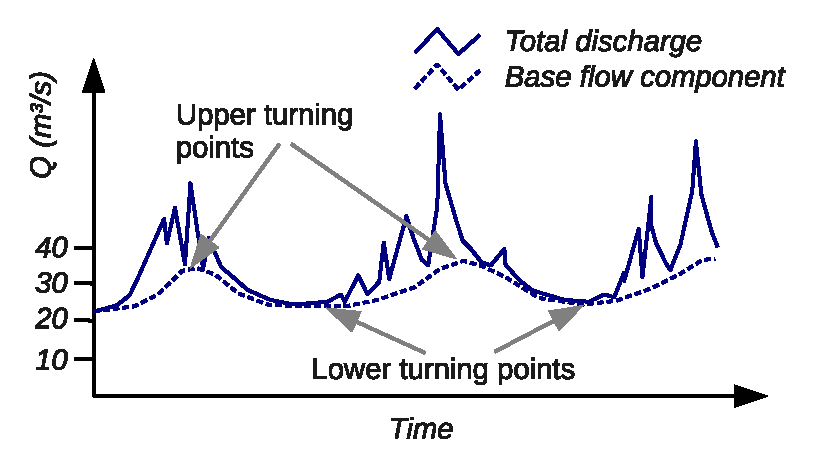
\includegraphics[width=0.9\columnwidth]{\figdir/parEstim_facBase.eps}
  \caption{Discharge hydrograph with manually separated base flow component. \label{fig:runGen4comp_parEstim_facBase}}
\end{figure}

In the following we assume that the base flow component is equivalent to the outflow from a conceptual ground water reservoir. For simplicity, we may consider a linear reservoir described by \eqnsref{eqn:runConcParStor_linResBalance} \& \ref{eqn:runConcParStor_linResOutflow} (see page \pageref{eqn:runConcParStor_linResBalance}). From the differential equation, we find that, at the mentioned turning points, the derivative of the storage volume with respect to time becomes zero, hence the rates of inflow and outflow are equal. Consequently, the \emph{base flow rate} at the turning points in a plot like \figref{fig:runGen4comp_parEstim_facBase} directly yields an estimate of the \emph{rate of ground water recharge}, \rateRunoffBase{}, at the respective point in time.

The relation between the actual rate of ground water reacharge \rateRunoffBase{} and the model parameter \facBase{} is given by \eqnref{eqn:runGen4comp_baseRunoff}. This can be rearranged and \rateRunoffBase{} can be substituted by $A \cdot Q_{base}$ where $A$ is the size of the catchment in units of \sqm{} and $Q_{base}$ is the base flow component in \cbms{} (\eqnref{eqn:runGen4comp_parEstim_facBase}). Using the fixed values of \relSatBase{} and \expBase{} mentioned in  \secref{sec:runGen4comp_processes}, we end up with \eqnref{eqn:runGen4comp_parEstim_facBase_final}.

\begin{eqnarray}
  \facBase &=& \dfrac{Q_{base}}{A} \cdot \left( \dfrac{\relSat-\relSatBase}{1 - \relSatBase} \right) ^ {-\expBase} \label{eqn:runGen4comp_parEstim_facBase} \\
           &=& \dfrac{Q_{base}}{A} \cdot \left( \dfrac{0.95}{\relSat - 0.05} \right) \label{eqn:runGen4comp_parEstim_facBase_final}
\end{eqnarray}

In order to calculate \facBase{} from \eqnref{eqn:runGen4comp_parEstim_facBase_final} we have to supply an estimate of the soil saturation \relSat{} at the respective point in time (\ie{} the analyzed turning point). For the lower turning points, a reasonable guess can be obtained from the soil water content at the wilting point. For a silty soil, for example, the saturation \relSat{} would be $\approx$ 0.2 for a soil moisture at the wilting point of 0.1 and a maximum water content of 0.48 (see \tabref{tab:et:real:soilmoisture} on page~\pageref{tab:et:real:soilmoisture}).

The value of \facBase{} obtained from the hydrograph analysis is a crude estimate. However, it might help in the definition of a proper search range for \facBase{} in the context of automatic model calibration.
